\label{sl-nn}
In this chapter we will make a an overview about neural networks and some other concepts  for better explain the following parts of the thesis.

\section{Introduction}
The Artificial Neural Networks is a family of classification technique\footnote{Classification is the operation of learning a function \textbf{$f$} that map example records \textbf{$x \in D$}, where $D$ is the set of \textbf{$(x, y)$}, to the labels set \textbf{$y$} (the classes). This target function is called also Classification Model and is used in a descriptive or predictive way problem depending.}, that are inspired by the human brain: in particular by the connections inside this latter. The human brain consists principally of nerve cells called \textbf{neurons}, that are connected together via the \textbf{axons}\footnote{Inserirne una, se serve} used to transmit the electrical impulse by a neuron to another. This electrical impulse generated by a stimulated neuron is transferred to another one via the dendrites, a particular elements in the human brain used to connect two neuron: this point of contact is called synapse. \newline Analogously the internal structure of a Neural Network is composed by components, which are called \textbf{neurons}, connected together by directed links. There are many types of Neural Networks, but for the sake of simplicity and  for the scope of the thesis we will focus the attention to feedforward neural network model, explaining firstly the Perceptron model.

\section{Perceptron}\label{sec:perceptron}
The Perceptron model is the basic and simplest type of Neural Network, proposed firstly by Frank Rosenblatt in 1958. This model is composed only by two types of nodes called \textbf{input nodes} and \textbf{output node}, as illustrated in the figure \ref{fig:illustration-perceptron-model}. As we can see in this latter the input nodes and the output node are connected by weighted links, similarly to the human brain, that are used to simulate the synaptic connections strength. \newline
\begin{figure}[t]
	\centering

	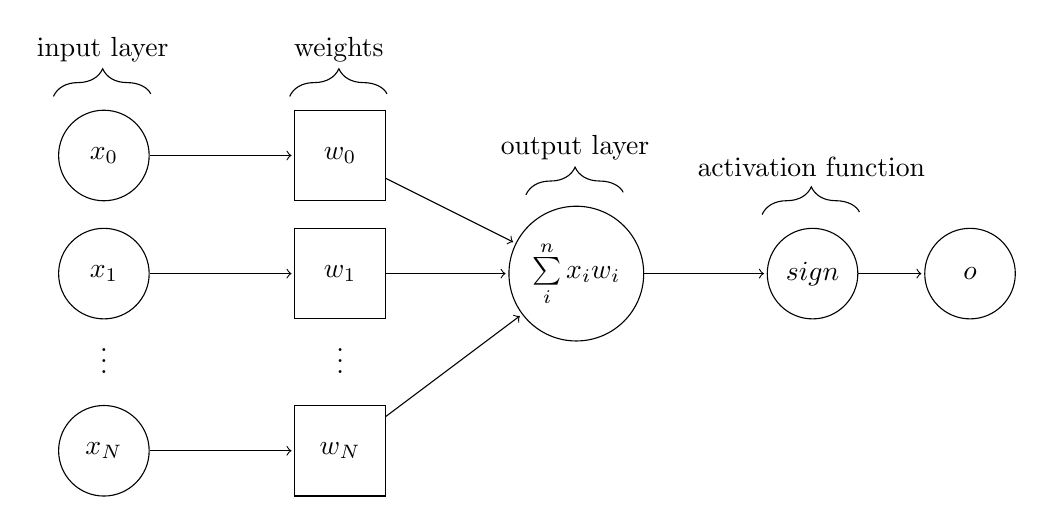
\begin{tikzpicture}[shorten >=1pt]
		\tikzstyle{unit}=[draw,shape=circle,minimum size=1.15cm]
		%\tikzstyle{hidden}=[draw,shape=circle,fill=black!25,minimum size=1.15cm]
		\tikzstyle{hidden}=[draw,shape=circle,minimum size=1.15cm]
		\tikzstyle{weights}=[draw,shape=rectangle,minimum size=1.15cm]

		\node[unit](x0) at (0,3.5){$x_0$};
		\node[unit](x1) at (0,2){$x_1$};
		\node at (0,1){\vdots};
		\node[unit](xd) at (0,-0.25){$x_N$};

		\node[weights](w0) at (3,3.5){$w_0$};
		\node[weights](w1) at (3,2){$w_1$};
		\node at (3,1){\vdots};
		\node[weights](wd) at (3,-0.25){$w_N$};

		\node[unit](y1) at (6, 2){$\sum\limits_{i}^{n}{x_iw_i}$};

		\node[unit](f) at (9, 2){$sign$};
		
		\node[unit](o) at (11, 2){$o$};

		\draw[->] (x0) -- (w0);
		\draw[->] (x1) -- (w1);
		\draw[->] (xd) -- (wd);
		
		\draw[->] (w0) -- (y1);
		\draw[->] (w1) -- (y1);
		\draw[->] (wd) -- (y1);

		\draw[->] (y1) -- (f);
		
		\draw[->] (f) -- (o);
			
		\draw [decorate,decoration={brace,amplitude=10pt},xshift=-4pt,yshift=0pt] (-0.5,4.25) -- (0.75,4.25) node [black,midway,yshift=+0.6cm]{input layer};
		\draw [decorate,decoration={brace,amplitude=10pt},xshift=-4pt,yshift=0pt] (2.5,4.25) -- (3.75,4.25) node [black,midway,yshift=+0.6cm]{weights};
		\draw [decorate,decoration={brace,amplitude=10pt},xshift=-4pt,yshift=0pt] (5.5, 3) -- (6.75, 3) node [black,midway,yshift=+0.6cm]{output layer};
		\draw [decorate,decoration={brace,amplitude=10pt},xshift=-4pt,yshift=0pt] (8.5, 2.75) -- (9.75, 2.75) node [black,midway,yshift=+0.6cm]{activation function};
	\end{tikzpicture}
	\caption{Illustration of the Perceptron model}\label{fig:illustration-perceptron-model}
\end{figure}	


This model calculate the output $\hat{y}$ as a weighted sum of the input respect to the connections weight, to which is summed the bias (a value used to rectify, in this case, the neural network output). So recalling some math, the output of the Perceptron model can be expressed in the following way:
\begin{center}
	$\hat{y} = \textbf{g}(w_{0}x_{0} + w_{1}x_{1} + \dots + w_{i-1}x_{i-1}  + w_{i}x_{i} + b  ) = \textbf{g}(\textbf{w} \bullet \textbf{x})$
\end{center}
where $i = 1, \dots, N$ and $N$ is the cardinality of the vector $\textbf{x}$ and the $\textbf{g}$ acts as the activation function\ref{fig:activation-functions}.
The training of a Perceptron neural network consist in recalculate (the key passage at the step 7 of algorithm \ref{alg:perceptron-learning}), or more precisely adapting, in an iterative manner the weight of the connections until they are able to fit the input data, i.e. the examples $(x, y) \in D$, minimizing or maximizing an objective function.
At the step 7 of the algorithm \ref{alg:perceptron-learning}
\begin{center}
	$w_{j}^{(k + 1)} = w_{j}^{(k)} + \lambda(y_{i} + \hat{y}_{i}^{(k)})x_{ij}$	
\end{center}
we can recognize the $w_{j}^{(k)}$ that is the connection weight of this step, $\lambda$ is the learning rate which is a parameter that instruct the learning algorithm how much quickly the neural network must abandons the old beliefs to substitute them with the new ones and $x_{ij}$ that is the $j^{th}$ value of the $i^{th}$ example.

\begin{algorithm}
	\begin{algorithmic}[1]
		\State{Let $D = \{(\textbf{x}_i, y_i)\ |\ i  = 1, \dots, N\}$ be the set of examples.}
		\State{Initialize the weight vector with random values, $\textbf{w}^{(0)}$}
		\Repeat
			\For{ each example $(\textbf{x}_{i}, y_{i}) \in D$}
				\State Compute the predicted output $\hat{y}_{i}^{(k)}$
				\For{ each weight $w_i$}
					\State Update the weight $w_{j}^{(k + 1)} = w_{j}^{(k)} + \lambda(y_{i} + \hat{y}_{i}^{(k)})x_{ij}$
				\EndFor
			\EndFor
		\Until{ Stopping condition is met }
	\end{algorithmic}
	\caption{Perceptron learning algorithm\cite{ITDM:2014}}\label{alg:perceptron-learning}
\end{algorithm}

\section{Multi-Layer Perceptron (MLP)}
The multilayer perceptron, known as feedforward neural networks, can be seen as an evolution of single layer perceptron\ref{sec:perceptron}, principally created to resolve the problem that this latter has because:
\begin{itemize}
	\item[•] It can not handles a domain $(\textbf{x}, y) \in D$ with more than two classes, because it divides the input data in only two boundaries, as it can be seen in the figure \ref{fig:perceptron-boundaries}, so more dimensions can not be handled
	\item[•] It can not converge if the data is not linearly separable and this leads to reduce the use of Perceptron in many few case (trivially when the data is linearly separable)
\end{itemize}

\begin{figure}[t!]
	\centering
	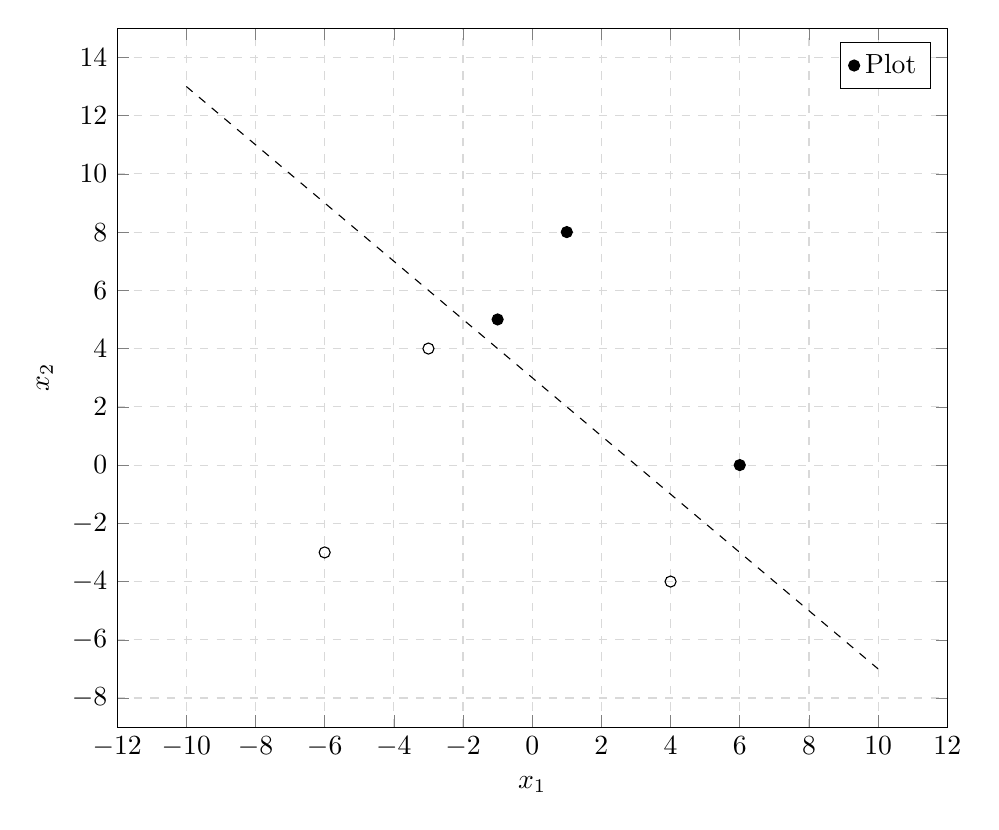
\begin{tikzpicture}
		\begin{axis}[
			width=\linewidth, % Scale the plot to \linewidth
    	     	grid=major, % Display a grid
    	      	grid style={dashed,gray!30}, % Set the style
			xlabel=$x_1$,
			ylabel=$x_2$,
		    %xtick=\empty, ytick=\empty
		]
		\addplot [only marks] table {
			1 8
			6 0
			-1 5
		};
		
		\addplot [only marks, mark=o] table {
			-6 -3
			4 -4
			-3 4
		};
		\addplot [domain=-10:10, samples=2, dashed] {-x + 3};

        \legend{Plot}
      \end{axis}
	\end{tikzpicture}
	\caption{Representation of decisione separation of a perceptron.}\label{fig:perceptron-boundaries}
\end{figure}

As the Perceptron the goal of MLP is to approximate a function $f^{*}$ that should represent the underlying data with which the neural network is trained, e.g. a classifier where $y=f^{*}(\textbf{x})$ associate an example record $\textbf{x}$ to class $y$. \newline \newline
These models, that includes also single layered perceptron, are called feedforward because the informations flow through the input layer, that contains the data from the example \textbf{x}, through all the intermediate layers called \textbf{hidden layer} and finally to the output layer $\textbf{y}$. So all these levels are connected only with next  and what is missing are feedback connections that fed back the network with the output of neural network, exclusive characteristic of others neural networks called \textbf{recurrent neural networks}. 

To all of these layer are associated different functions, called \textbf{activation function}, that permits to the layers to produce output values that are nonlinear respect the input parameters. Thus, in an other perspective, a feedforward neural networks can be seen as a chain of activation functions.

\begin{figure}[t]
	\centering
	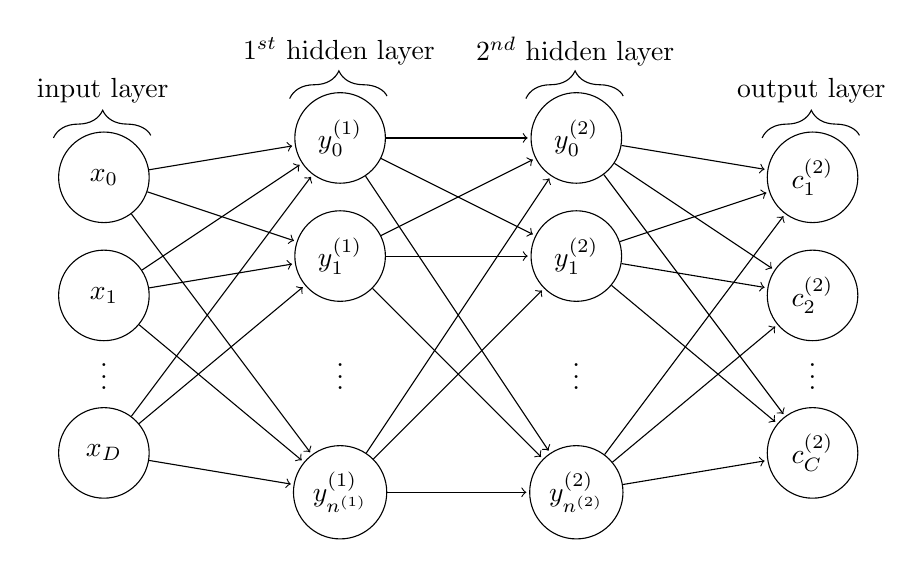
\begin{tikzpicture}[shorten >=1pt]
		\tikzstyle{unit}=[draw,shape=circle,minimum size=1.15cm]
		%\tikzstyle{hidden}=[draw,shape=circle,fill=black!25,minimum size=1.15cm]
		\tikzstyle{hidden}=[draw,shape=circle,minimum size=1.15cm]

		\node[unit](x0) at (0,3.5){$x_0$};
		\node[unit](x1) at (0,2){$x_1$};
		\node at (0,1.075){\vdots};
		\node[unit](xd) at (0,0){$x_D$};

		\node[hidden](h10) at (3,4){$y_0^{(1)}$};
		\node[hidden](h11) at (3,2.5){$y_1^{(1)}$};
		\node at (3,1.075){\vdots};
		\node[hidden](h1m) at (3,-0.5){$y_{n^{(1)}}^{(1)}$};
		
		\node[hidden](hL0) at (6,4){$y_0^{(2)}$};
		\node[hidden](hL1) at (6,2.5){$y_1^{(2)}$};
		\node at (6,1.075){\vdots};
		\node[hidden](hLm) at (6,-0.5){$y_{n^{(2)}}^{(2)}$};

		\node[unit](y1) at (9,3.5){$c_1^{(2)}$};
		\node[unit](y2) at (9,2){$c_2^{(2)}$};
		\node at (9,1.075){\vdots};	
		\node[unit](yc) at (9,0){$c_C^{(2)}$};

		
		\draw[->] (x0) -- (h10);
		\draw[->] (x0) -- (h11);
		\draw[->] (x0) -- (h1m);

		\draw[->] (x1) -- (h10);
		\draw[->] (x1) -- (h11);
		\draw[->] (x1) -- (h1m);

		\draw[->] (xd) -- (h10);
		\draw[->] (xd) -- (h11);
		\draw[->] (xd) -- (h1m);

		\draw[->] (hL0) -- (y1);
		\draw[->] (hL0) -- (y2);
		\draw[->] (hL0) -- (yc);

		\draw[->] (hL1) -- (y1);
		\draw[->] (hL1) -- (y2);
		\draw[->] (hL1) -- (yc);

		\draw[->] (hLm) -- (y1);
		\draw[->] (hLm) -- (y2);
		\draw[->] (hLm) -- (yc);

		\draw[->] (h10) -- (hL0);
		\draw[->] (h11) -- (hL0);
		\draw[->] (h1m) -- (hL0);
		
		\draw[->] (h10) -- (hL1);
		\draw[->] (h11) -- (hL1);
		\draw[->] (h1m) -- (hL1);
		
		\draw[->] (h10) -- (hLm);
		\draw[->] (h11) -- (hLm);
		\draw[->] (h1m) -- (hLm);
		
		\draw [decorate,decoration={brace,amplitude=10pt},xshift=-4pt,yshift=0pt] (-0.5,4) -- (0.75,4) node [black,midway,yshift=+0.6cm]{input layer};
		\draw [decorate,decoration={brace,amplitude=10pt},xshift=-4pt,yshift=0pt] (2.5,4.5) -- (3.75,4.5) node [black,midway,yshift=+0.6cm]{$1^{\text{st}}$ hidden layer};
		\draw [decorate,decoration={brace,amplitude=10pt},xshift=-4pt,yshift=0pt] (5.5,4.5) -- (6.75,4.5) node [black,midway,yshift=+0.6cm]{$2^{\text{nd}}$ hidden layer};
		\draw [decorate,decoration={brace,amplitude=10pt},xshift=-4pt,yshift=0pt] (8.5,4) -- (9.75,4) node [black,midway,yshift=+0.6cm]{output layer};
	\end{tikzpicture}
	\caption[Graph representation of feedforward neural network.]{Graph representation of feedforward neural network with $(2)$-layer, with $D$ input units and $C$ output units. Every layer contains $n^(i)$ neurons, where $i$ is the index of the level.}
	\label{fig:multilayer-perceptron}
\end{figure}

From this description we can see that the major difference between single-layered perceptron and feedforward neural networks is the training strategy. In fact the design of the FFN prevents to approach the training with the same strategy used with the perceptron because we does not have \textit{a priori} the informations regard the desired output of all the hidden layers, so we can not update the weights as we have seen in the perceptron.

\section{Artificial Neural Network training} 
Leaving out the specific training of the perceptron, that is treated shortly previously, the training of a ANN generally follow two main steps: the initialization of the weights and the recalculation of these latter with an algorithm that is guided by the objective to minimize or maximize an objective function\footnote{In specific we speak of cost or loss function if the objective is to minimize this latter.}.

The specific operations in the second step are variable and depend by the used algorithm, but generally can be subdivided in two more sub-steps: firstly is calculated the objective function with which, in the second steps, all the weights are recalculated with some strategy/algorithm. The most famous technique to do this is the backpropagation, that we present in the subsection \ref{subsec:backpropagation}, but is not the only one that exists (as we show in the section \ref{chap:differential-evolution}) and that we have treated in this thesis work.

\subsection{Backpropagation}\label{subsec:backpropagation}
Backpropagation is an algorithm introduced in \cite{RUM:1986} used to calculate the contribution in error of each neuron for a batch of data computed with respect to an objective function. This latter must be a function that can be capture the difference between the expected output, i.e. the $y$ associated to each example, and the generated output, i.e. the $\hat{y}$ associated to each example, transforming that in a real value.
An example of objective function is the Total Sum of Squared errors:
\begin{center}
$TSS = \frac{1}{2}\sum\limits_{i=1}^{N}(y_i - \hat{y}_{i})^{2}$
\end{center}
The backpropagation is divided into two phase, the forward propagation and the backward propagation.

\subsubsection{Forward propagation}
Intuitively in the forward propagation pass the network is "forward executed", i.e. starting from the input example the calculations for all the layers are executed up to the output layer in a forward manner. \\
Formally let $D = \{(\textbf{x}, y)_i\ |\ i=1, \dots, n \}$ the set of examples where $\textbf{x} = \{x_1, x_2, \dots, x_n\}$ is an example and $y$ is the associated class, $H = \{h^{(j)}\ |\ j = 1, \dots, M\}$ the set of FNN hidden layers and $B = \{b^{(j)}\ |\ j=1, \dots, M\}$ the set of bias vectors. Then in this phase the parameters, i.e. the weights, for the first level are calculated in this way
\begin{center}
	$h^{(1)} = \Theta^{(1)}(\sum\limits_{i=1}^{|\textbf{x}|}{x_{i}h^{(1)}_{i}} + b^{(1)})$
\end{center}
where $\Theta^{1}$ is the activation function of the first layer.\\
Then, as state previously, the computation continue forward for all the others hidden layers as follow
\begin{center}
	$h^{(j)} = \Theta^{(j)}(\sum\limits_{i \in h^{(j - 1)}}h_{i}^{(j - 1)}h_{i}^{(j)} + b^{(j)})$
\end{center}
where the $h^{(j - 1)}$ are the calculated weights of the previous layer of the layer $h^{(j)}$, up to the output layer where we have
\begin{center}
	$\hat{y} = \Theta^{(M)}(\sum\limits_{i \in C}h_{i}^{(M - 1)}h_{i}^{(M)} + b^{(M)})$
\end{center}
where $\hat{y}$ is the neural networks output that will be used in the backward propagation step.

\subsubsection{Backward propagation}

A strictly requirement of backpropagation is that all the activation functions must be differentiable, otherwise is demonstrated that this algorithm will not converge.

%\section{Recurrent neural networks}
% Write this section if there is remaining time